\documentclass[12pt]{article}
\usepackage[utf8]{inputenc}
\usepackage[a4paper, margin=2cm]{geometry}
\usepackage{multicol, caption}
\usepackage{authblk}
\usepackage[varg]{txfonts}
\usepackage{titlesec}
%\usepackage[T1]{fontenc}
%\usepackage{lmodern}
% \usepackage[english]{babel}


\usepackage{amsmath}
\usepackage{amssymb}
\usepackage{amsfonts}
\usepackage{graphicx}% Include figure files
\usepackage{dcolumn}% Align table columns on decimal point
\usepackage{bm}% bold math
\usepackage{hyperref}% add hypertext capabilities
\usepackage{minted}
\usepackage[autostyle]{csquotes}
\usepackage{wrapfig}

\usepackage[backend=biber,style=numeric]{biblatex}
\addbibresource{bib.bib}

\hyphenpenalty=10000
\exhyphenpenalty=10000

% CUSTOM FORMAT FOR SECTION
\titleformat{\section}[wrap]{\normalfont\bfseries}{\thesection.}{0.5em}{}
\titlespacing{\section}{12pc}{1.5ex plus .1ex minus .2ex}{1pc}
% CUSTOM SUBSECTION
\titleformat{\subsection}[wrap]{\normalfont\bfseries}{\thesubsection.}{0.5em}{}
\titlespacing{\subsection}{12pc}{1.5ex plus .1ex minus .2ex}{1pc}
% CUSTOM SUBSUBSECTION 
\titleformat{\subsubsection}[wrap]{\normalfont\bfseries}{\thesubsubsection.}{0.5em}{}
\titlespacing{\subsubsection}{12pc}{1.5ex plus .1ex minus .2ex}{1pc}

% CUSTOM LINE SPACING (Default 1.2 -> 1.2*1.25=1.5)
\linespread{1.25}

% CUSTOM NAMING
\renewcommand*\contentsname{Summary}

% CUSTOM FIGURES
\usepackage{import}
\usepackage{xifthen}
\usepackage{pdfpages}
\usepackage{transparent}
\newcommand{\incfig}[2][1]{
    \def\svgwidth{#1\textwidth}
    \input{#2.pdf_tex}
}

%CUSTOM APPENDIX
\usepackage[toc, page]{appendix}

\newenvironment{Figure}
  {\par\medskip\noindent\minipage{\linewidth}}
  {\endminipage\par\medskip}

\title{PHYS6006 Project Summary Report \\
       Magnetospheric Structure Associated with High-Latitude Auroras}
\author{J. Plank}

\begin{document}\sloppy
% TITLE BLOCK
\maketitle

% ABSTRACT
% \begin{abstract}
%     \noindent\textit{Context:} Current understanding of the magnetospheric structure associated with the formation of high latitude auroras is limited to case studies only, and the connection to interplanetary magnetic field (IMF) direction is suspected but has never been quantified.\\
%     \textit{Aims:} To produce a statistical appraisal of the relationship between a northward pointing IMF and a phenomenon known as transpolar arcs.\\
%     \textit{Methods:} Using data from the ESA satellite Cluster and NASA's OMNI dataset, the average IMF $B_Z$ at high temperatures $T>20\ MK$ at increasing $Z$, covering the plasma sheet and the lobe was analysed. \\
%     \textit{Results:} There is no general correlation between high temperatures in the lobe and the presence of northward IMF. There were, however, several occasions when a connection was present (2002 and 2005), which merit further exploration.
% \end{abstract}

% \pagebreak

% \tableofcontents
% \addtocontents{toc}{~\hfill\textbf{Page}\par}

% \pagebreak

% % SWITCH TO 2 COLUMNS
% \begin{multicols}{2}

The northern lights are a beautiful yet complex natural phenomenon arising from interactions within the enormous, invisible, field of magnetic energy between the Sun and the Earth. The Earth’s molten iron core generates enormous loops of magnetic field that stretch out into space over a distance equivalent to several times the diameter  of the planet. The Sun has an even more powerful magnetic field which causes its surface to writhe and boil, ejecting highly energetic plasma out into the space between planets, which in turn pulls the magnetic field of the Sun out even further into space. 

This far-reaching field from the Sun, known as the interplanetary magnetic field (IMF), stretches far enough to collide with planet Earth - or it would, if our own magnetic field was not  there to block it and shield us from potentially harmful radiation. 

The Sun - being essentially a giant nuclear bomb - is very volatile, and as such, its magnetic field is much less consistent than Earth’s. Magnetic fields always have a direction, and in the Sun that direction can change polarity on a regular basis, especially at the equator. Earth experiences the full effect of this changeability since it orbits in a circle that traces an almost perfect line around the Sun’s equator, which results  in the IMF, when measured at Earth, sometimes pointing northwards, and sometimes southwards. 

When it points southwards, it can merge with Earth’s field (which, confusingly, flows from the south pole to north) in a process known as reconnection, pictured in Figure 1, where IMF field lines (blue) merge with the field lines of Earth (red). This allows the energetic plasma from the Sun to be transmitted down to the atmosphere, where it collides with particles in the air, causing an explosion of light which we see as auroras, often described as ‘curtains’ of  light ‘dancing’ through our atmosphere. However, this type of reconnection cannot happen during the times when the interplanetary magnetic field points northward. Instead, we sometimes see a special type of aurora known as a transpolar arc. These do not  appear in the usual oval at roughly $70^\circ$ latitude, but instead cross right up into the polar cap itself. 

\begin{figure}
    \centering
    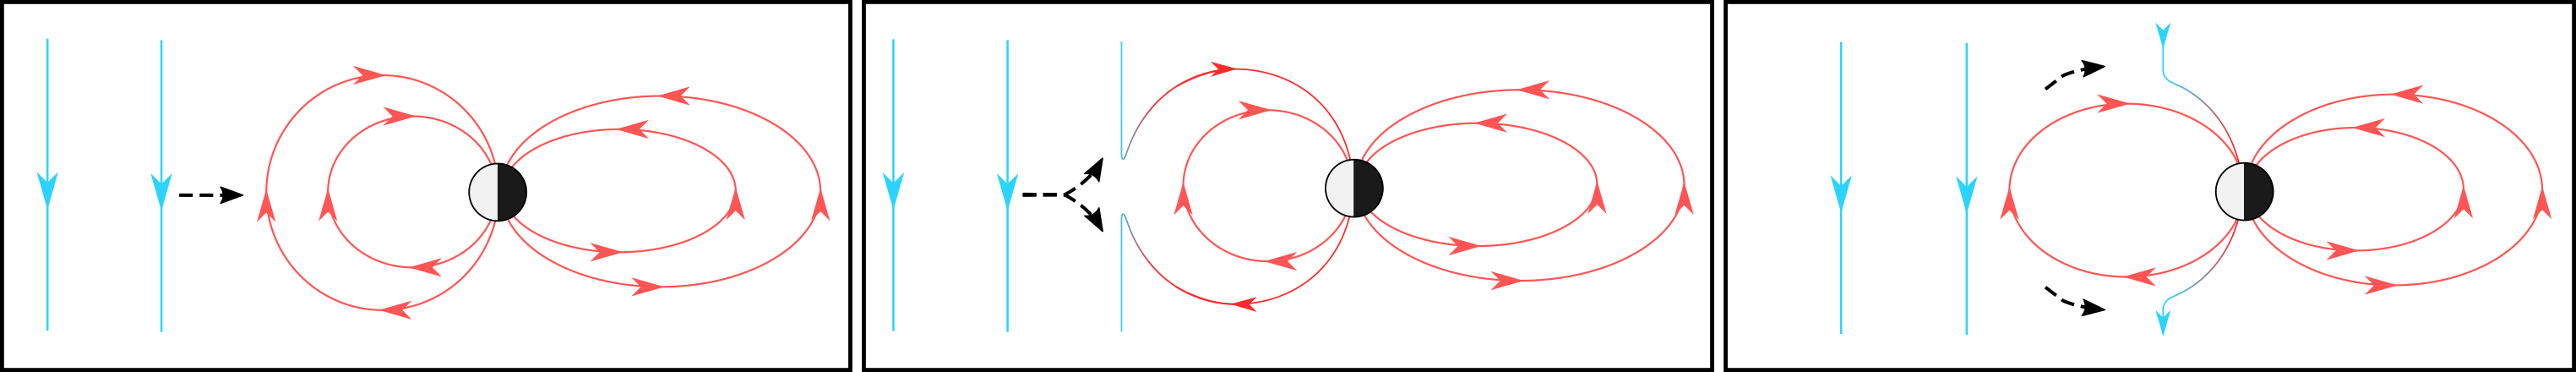
\includegraphics[width=\textwidth]{DungeyCycle.png}
    \caption{Simplified picture of reconnection happening on the daytime side of the planet. IMF field lines from the Sun (pictured in blue) move horizontally towards the field lines of Earth that flow in the opposite direction. Reconnection causes them to merge together which allows the Sun’s plasma to reach Earth and cause aurora. }
    \label{fig:dungey}
\end{figure}

There are significant gaps in our understanding of  northwards pointing IMF,  including the phenomenon of transpolar arcs. One theory \cite{TPAdebate} suggests that, although dayside reconnection cannot happen, the equivalent night-side reconnection that closes the loop again remains possible, causing   a build-up of energy that cannot move back around to the front of the planet to begin another cycle of reconnection. It has nowhere to go but to spread out upwards and downwards, into an area of Earth’s field known as the lobes. 

If this were the case, when we compare areas of high temperature in the lobes\footnote{Using data from ESA's Cluster satellites} to the direction of the IMF\footnote{data from NASA (OMNI)}, there would be an increase in the presence of northwards IMF as vertical distance above/below the planet is increased. 

But, when this relationship was examined the result was not so clear. There were some periods (late 2002 and late 2005) where the result very strongly suggested that this was indeed the case, but most other times showed that there was no significant increase in northwards IMF when examining high temperatures in the lobe. 

These periods of high temperature were also compared to images of the aurora itself, as a way of checking another step in the predicted chain of northwards IMF causing high temperatures in the lobe, causing transpolar arcs. It was discovered that a transpolar arc occurred in 50\% of predicted occasions, and 50\% of those happened when the IMF was pointing northwards. Further research is warranted because this result has demonstrated exciting activity in an area previously considered of lesser consequence.

\printbibliography

\end{document}
